% !TeX TXS-program:compile = txs:///arara
% arara: lualatex: {shell: no, synctex: yes, interaction: batchmode}
% arara: pythontex: {rerun: modified} if found('pytxcode', 'PYTHONTEX#py')
% arara: lualatex: {shell: no, synctex: yes, interaction: batchmode} if found('pytxcode', 'PYTHONTEX#py')
% arara: lualatex: {shell: no, synctex: yes, interaction: batchmode} if found('log', '(undefined references|Please rerun|Rerun to get)')

\documentclass[a4paper,11pt]{article}
\usepackage[revgoku]{cp-base}
\graphicspath{{./graphics/}}
%variables
\donnees[classe={1\up{ère} 2M2},matiere={[SPÉ.MATHS]},mois=Avril,annee=2022,typedoc=CHAP,numdoc=10]
%formatage
\author{Pierquet}
\title{\nomfichier}
\hypersetup{pdfauthor={Pierquet},pdftitle={\nomfichier},allbordercolors=white,pdfborder=0 0 0,pdfstartview=FitH}
%divers
\lhead{\entete{\matiere}}
\chead{\entete{\lycee}}
\rhead{\entete{\classe{} - \mois{} \annee}}
\lfoot{\pied{\matiere}}
\cfoot{\logolycee{}}
\rfoot{\pied{\numeropagetot}}

\begin{document}

\pagestyle{fancy}

\part{CH10 - Calcul vectoriel, produit scalaire - Exercices}

\medskip

\begin{caide}
{\setlength\arrayrulewidth{1.5pt} \arrayrulecolor{titrebleu!35}
\begin{tabularx}{\linewidth}{Y|Y|Y|Y|Y|Y}
	\niveaudif{0}~~\textsf{Basique} & \niveaudif{1}~~\textsf{Modérée} & \niveaudif{2}~~\textsf{Élevée} & \niveaudif{3}~~\textsf{Très élevée} & \niveaudif{4}~~\textsf{Extrême} & \niveaudif{5}~~\textsf{Insensée} \\
\end{tabularx}}
\end{caide}

\exonum{0}

\begin{enumerate}
	\item Déterminer $\vect{AB}\cdot\vect{AC}$ avec comme données $AB=4$ ; $AC=3$ et $\widehat{BAC}=60^{\circ}$.
	\item Déterminer $\vect{AB}\cdot\vect{AC}$ avec les données suivantes :
	\begin{center}
		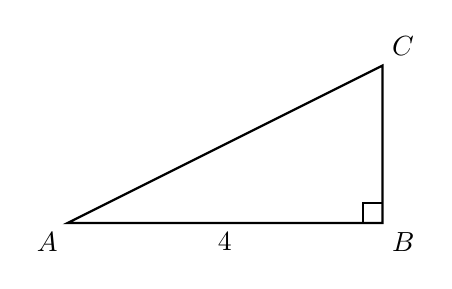
\begin{tikzpicture}
			\draw[thick] (0,0)--(4,0)--(4,2)--cycle;
			\draw (0,0) node[below left] {$A$} ;
			\draw (4,0) node[below right] {$B$} ;
			\draw (4,2) node[above right] {$C$} ;
			\draw[thick] (3.75,0) |- (4,0.25) ;
			\draw (2,0) node[below] {$4$} ;
		\end{tikzpicture}
	\end{center}
	\item Déterminer $\vect{u}\cdot\vect{v}$ puis $\vect{u}^2$ puis $\vect{v}^2$ avec comme données $\vec{u}\coordeux{4}{-1}$ et $\vec{v}\coordeux{3}{5}$.
\end{enumerate}

\medskip

\exonum{1}

\medskip

On se place dans un repère orthonormal $\Rij$.

\begin{enumerate}
	\item On donne $\vec{u}\coordeux{1}{2}$ et $\vec{v}\coordeux{-6}{3}$. Les vecteurs $\vect{u}$ et $\vect{v}$ sont-ils colinéaires ? orthogonaux ? Justifier.
	\item On considère les points $A\coordpl{1}{3}$, $B\coordpl{-2}{7}$ et $C\coordpl{9}{9}$.
	\begin{enumerate}
		\item Déterminer les coordonnées des vecteurs $\vect{AB}$ et $\vect{AC}$.
		\item Calculer $\vect{AB}\cdot\vect{AC}$.
		\item En déduire la nature du triangle $ABC$.
	\end{enumerate}
\end{enumerate}

\medskip

\exonum{1}

\medskip

Les côtés des carrés accolés $ABCD$ et $BEFC$ ont pour longueur 3. $I$ est l'intersection des segments $[AF]$ et $[BC]$.

\begin{center}
	\begin{tikzpicture}[thick]
		\draw[thick] (0,0) rectangle (6,3);
		\draw[->,>=stealth'] (0,0)--(1,0) ;
		\draw[->,>=stealth'] (0,0)--(0,1) ;
		\draw (0,0) node[below left] {$A$} ; \draw (3,0) node[below] {$B$} ; \draw (6,0) node[below right] {$E$} ;
		\draw (0,3) node[above left] {$D$} ; \draw (3,3) node[above] {$C$}  ; \draw (6,3) node[above right] {$F$} ;
		\draw (0,0) -- (6,3) (3,0)--(3,3);
		\draw (0,1.5) node[left] {$3$} ;
		\draw (3,1.65) node[left] {$I$} ;
	\end{tikzpicture}
\end{center}

\begin{enumerate}
	\item 
	\begin{enumerate}
		\item Calculer la longueur $AF$ puis en déduire une valeur de $\cos\left(\widehat{EAF}\right)$.
		\item En déduire une valeur de $\vect{AE}\cdot\vect{AI}$.
	\end{enumerate}
	\item En utilisant la formule du produit scalaire avec la projection orthogonale, retrouver le résultat $\vect{AE}\cdot\vect{AI}$.
	\item On se place dans le repère orthonormal $\left(A\,;\,\dfrac{1}{3}\vect{AB}\,,\,\dfrac{1}{3}\vect{AD}\right)$.
	\begin{enumerate}
		\item Déterminer les coordonnées des vecteurs $\vect{AE}$ et $\vect{AI}$.
		\item Retrouver la valeur de $\vect{AE}\cdot\vect{AI}$.
	\end{enumerate}
\end{enumerate}

\pagebreak

\exonum{1}

\medskip

Déterminer les éventuelles valeurs du réel $x$ pour lesquelles les vecteurs $\vect{u}$ et $\vect{v}$ sont orthogonaux :
\begin{multicols}{2}
	\begin{enumerate}
		\item $\vect{u}\coordeux{6}{x}$ et $\vect{v}\coordeux{-3}{2}$ ;
		\item $\vect{u}\coordeux{-3}{x}$ et $\vect{v}\coordeux{x-1}{4}$ ;
		\item $\vect{u}\coordeux{3}{8}$ et $\vect{v}\coordeux{x}{-2}$ ;
		\item $\vect{u}\coordeux{x}{2}$ et $\vect{v}\coordeux{x}{8}$.
	\end{enumerate}
\end{multicols}

\medskip

\exonum{2}

\medskip

Dans cet exercice, on va utiliser \calgpython{} pour étudier l'éventuelle orthogonalité de deux vecteurs $\vect{u}$ et $\vect{v}$ dont on connaît les coordonnées \cpy{xu}, \cpy{yu}, \cpy{xv} et \cpy{yv}.

\begin{envpython}[10cm]
	def produitscalaire(xu,yu,xv,yv) :
		res = ...............
		return res
	
	def orthogonaux(xu,yu,xv,yv):
		ps = produitscalaire(xu,yu,xv,yv)
		if ps .......... :
			return True
		else :
			return False
\end{envpython}

\begin{enumerate}
	\item Compléter la ligne \textsf{L2} de sorte que \cpy{res} contienne la valeur $\vect{u}\cdot\vect{v}$.
	\item Compléter la ligne \textsf{L7} de sorte que l'appel à la fonction \cpy{orthogonaux} renvoie \cpy{True} lorsque $\vect{u}\perp\vect{v}$ et \cpy{False} sinon.
	\item Que renvoie :
	\begin{enumerate}
		\item \cpy{produitscalaire(-1,5,4,3)} ?
		\item \cpy{orthogonaux(2,2.5,12.5,-10)} ?
	\end{enumerate}
\end{enumerate}

\medskip

\exonum{3}

\medskip

Le triangle isocèle $ABC$ est inscrit dans un trapèze rectangle $ABDE$. Les longueurs sont données en centimètre.

\begin{center}
	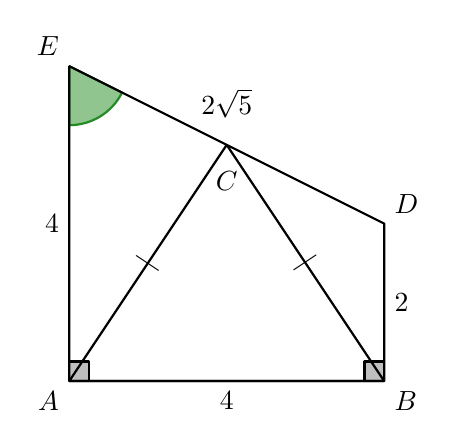
\begin{tikzpicture}[thick,line join=bevel]
		\draw[fill=lightgray] (0.25,0) rectangle (0,0.25) ; \draw[fill=lightgray] (3.75,0) rectangle (4,0.25) ;
		\draw[ForestGreen,fill=ForestGreen!50] (0,4) -- (0,3.25) arc (-90:-26.6:0.75) -- cycle;
		\draw (0,0) node[below left] {$A$} -- (4,0) node[below right] {$B$} -- (4,2) node[above right] {$D$} -- (0,4) node[above left] {$E$} -- cycle;
		\draw (0,0) -- (2,3) node[midway,sloped] {$|$} -- (4,0) node[midway,sloped] {$|$} -- cycle ;
		\draw (2,3) node[below=6pt] {$C$} ; \draw (2,3) node[above=6pt] {$2\sqrt{5}$} ;
		\draw (0,2) node[left] {$4$} ; \draw (2,0) node[below] {$4$} ; \draw (4,1) node[right] {$2$} ;
	\end{tikzpicture}
\end{center}

\begin{enumerate}
	\item 
	\begin{enumerate}
		\item Calculer, à l'aide d'une projection judicieuse, $\vect{AB}\cdot\vect{ED}$.
		\item Déterminer une valeur approchée, au dixième de degré, de la mesure de l'angle $\big( \vect{AB}\,,\,\vect{ED} \big)$.
		\item En déduire une valeur approchée, au dixième de degré, de la mesure de l'angle $\widehat{AED}$.
	\end{enumerate}
	\item 
	\begin{enumerate}
		\item Calculer $\vect{EA}\cdot\vect{EC}$.
		\item Grâce à la formule $\vect{u}\cdot\vect{v}=\tfrac{1}{2}\left(||\vect{u}||^2+||\vect{v}||^2-||\vect{u}-\vect{v}||^2\right)$, déterminer une valeur approchée, au dixième de centimètre, de la longueur $AC$.
	\end{enumerate}
\end{enumerate}

\end{document}